\section{Implementation}


\subsection{Model Adaptation}

\begin{figure}[tb]
	\centering
		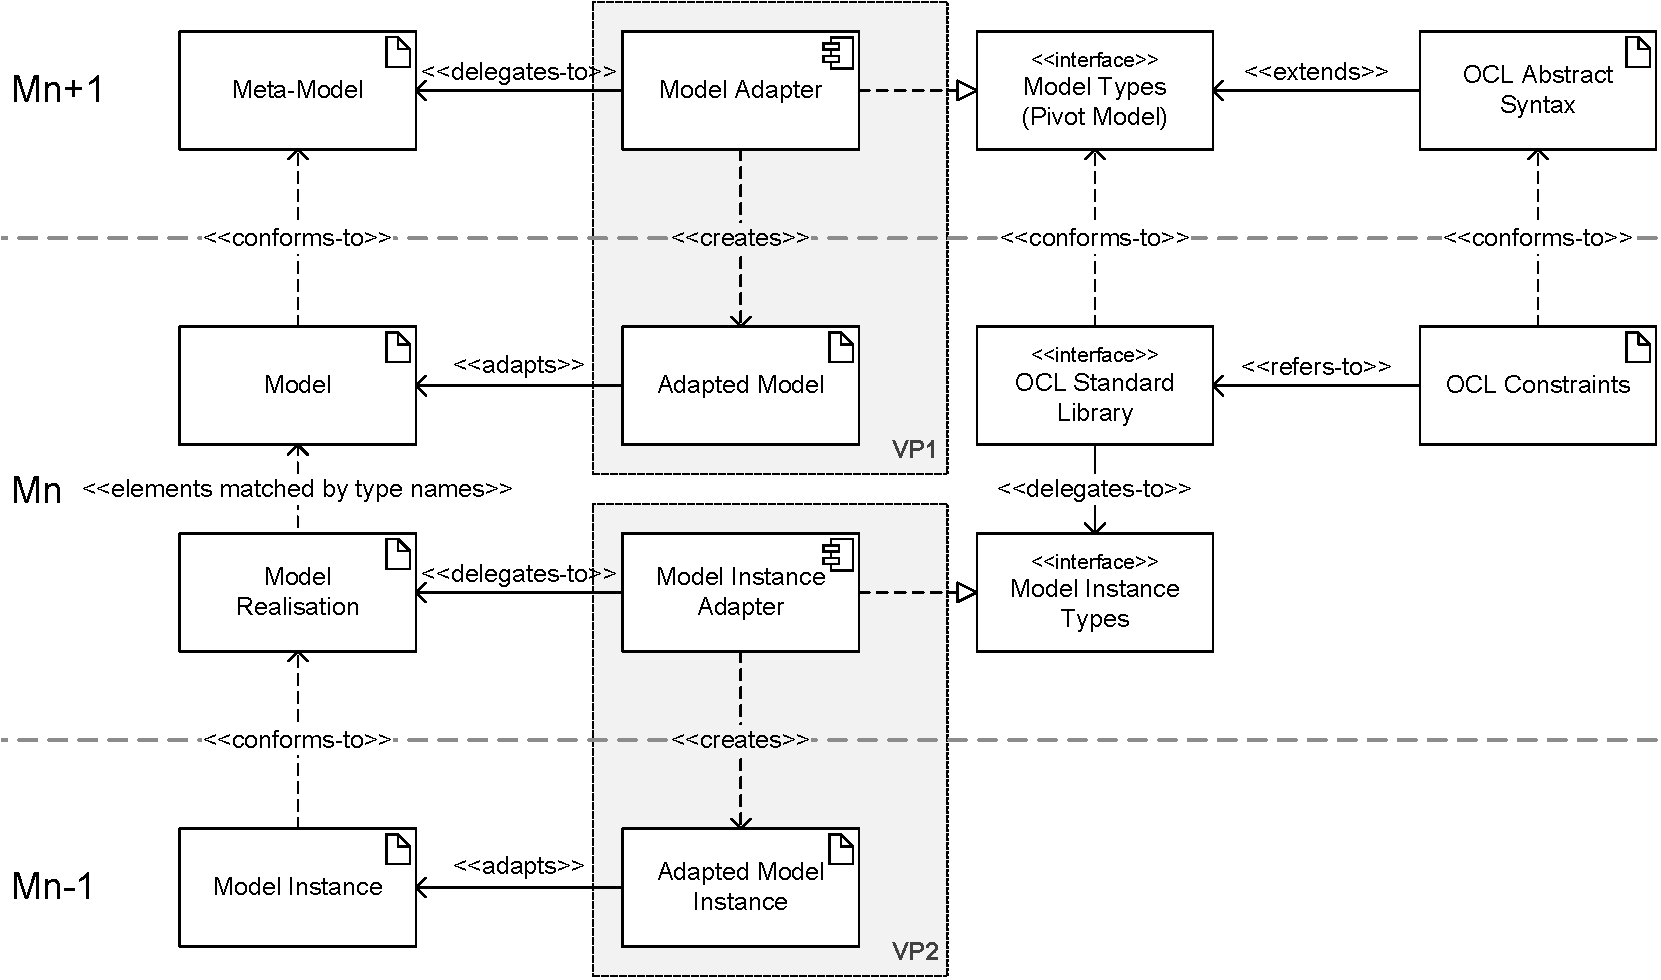
\includegraphics[width=1.00\textwidth]{figures/modeladaptation.pdf}
	\caption{The adaptation architecture of Dresden OCL2 for Eclipse. At the Mn+1 layer, meta-models are adapted to the pivot model. The adapter is responsible to wrap modeled models of the adapted meta-model as wrapped models as well. At the Mn layer, model implementation types can be adapted. Their adapter is responsible to wrap instances (or runtime objects) to wrapped model objects. The OCL standard library implements the logic to evaluate operation defined on OCL types. Other request such operation invocations or property request on wrapped objects are delegated via the interfaces of the model implementation type model.}
	\label{fig:modeladaptation}
\end{figure}

Handling different types of models behind common interfaces is the basis to define a generic OCL meta-model and abstract syntax that can be used to define and parse OCL constraints on different meta-models. Thus, Dresden OCL2 for Eclipse is based on a \textit{Pivot Model} designed by Matthias Br�uer \cite{braeuerOCL07} that abstracts the concepts of various meta-models such as the UML meta-model and the EMF Ecore meta-model. It describes the basic concepts that must be provided by a meta-model to define OCL constraints such as types, properties, operations and parameters.\footnote{All these concepts exist, but a meta-model can be adapted to a subset of these concepts as well. E.g, the XML meta-model XML-Schema cannot express operations. Nevertheless, it can be adapted to the pivot model.} The OCL tools only invoke the interfaces of the pivot model concepts when they want to reason on types defined in the adapted models (e.g. the OCL2 parser can invoke the operation \texttt{getType()} to reason the \texttt{Type} of an \texttt{Operation} or \texttt{Property}. Thus, the OCL2 Parser does not need to know the adapted meta-model and can be connected with different meta-models very easily.

For every meta-model that shall be connected with Dresden OCL2 for Eclipse, a \textit{Meta-Model Adapter} has to be implemented (see Figure \ref{fig:modeladaptation}, Mn+1 layer). The adapter contains implementations for all adapted pivot model elements (e.g., the UML meta-model element \texttt{UMLClass} is adapted to the pivot model element \texttt{Type}). Furthermore, the meta-model adapter contains a factory that creates adapters for currently accessed model elements (see Figure \ref{fig:modeladaptation}, Mn+1 and Mn layer). The model element adapters are only created when they are required and existing adapters are cached. Thus, we avoid unecessary and expensive adaptation, especially when working on large models of which only parts are constrained using OCL.


\subsection{Model Implementation Adaptation}

Similar to the adaptation of different meta-models and models (that can be considered as the specification or structure of a modeled system), it is also possible to adapt different kinds of implementations or semantics behind common interfaces to use the same OCL2 interpreter for the interpretation of OCL constraints on different types of model implementations. Furthermore, a specific model type can have different semantics in different implementations. E.g., a UML class diagram can be implemented in Java, C\#.\footnote{Although the implementation of the same model in different programming languages is rather unusual, it is often required to connect models of the same meta-model with different types of implementations.} Thus, it is sensible to loosely couple the models and their semantics. 

To fulfill these requirements, we designed a common \textit{Model Implementation Type Model} that can be adapted to different kinds of model implementations. The implementation type model can be considered as similar to the pivot model, but has some differences as well. Similar to the pivot model, the implementation type model defines different interfaces for different elements of an implementation such as instances of primitive types, enumeration literals, collections and instances of normal types defined in the model. All these interfaces inherit a common interface \textit{IModelInstanceElement}. The most important difference between the pivot model's and implementation type model's interfaces is that \texttt{IModelInstanceElements} have to provide a reflection mechanism whereas pivot model elements only allow to reason on relationship between elements of the same meta-level. During interpretation, the OCL2 interpreter must be able to reason on the Type of a \textit{IModelInstanceElement}, to retrieve property values and to invoke operations. The kind of reflection mechanism provided can be considered as similar to the Java reflections that allow to reason on types, to cast objects and to access properties and operations.

Each kind of model implementation that shall be connected with Dresden OCL2 for Eclipse has to be adapted via a \textit{Model Implementation Adapter} (see Figure \ref{fig:modeladaptation}, Mn layer). Similar to the meta-model adapter, the model implementation adapter has to provide adapters for the different concepts of the implementation type model and has to provide a factory that creates \textit{Model Object Adapters} for the runtime objects of the adapted implementation  (see Figure \ref{fig:modeladaptation}, Mn-1 layer). Similar to the meta-model factory, a model implementation factory only creates adapters for objects that are requested by the OCL2 interpreter during interpretation. Already adapted objects are cached to improve the performance and to avoid phenomenas like \textit{Object Schizophrenia}.


\subsection{Challenges}

During the implementation of our generic architecture that allows connection of different types of models with different types of model implementations and vice versa we had to focus on some problems and difficulties that are shortly presented in this section. 

As mentioned above, models and model implementations are only loosely coupled to support different implementations for the same type of model. Thus, we had to realize a matching algorithm that matches types of an implementation to the types of a given model. Currently, this type matching is realized by simply matching the names of the types (including the names of their enclosing name spaces where possible). Often, this solution is error prone and further information is hidden behind our adapters that could be used to improve the algorithm. E.g., when coupling an instance of an EMF Ecore model, Eclipse provides further mechanisms to reason on the types of EObjects. Thus, we plan to improve our matching algorithm that is currently scattered over multiple classes of each implementation type adapter and plan to introduce a set of type matching strategies that can be implemented based on the \textit{Chain of Responsibility} pattern\cite{gamma:dp}. The chain could start by trying to match the types using a implementation specific matcher and end by trying to simply match the type's names as currently done.

Another problem when using adapters for model implementation types is the unwrapping mechanism of adapted elements when invoking operations on the implementation's elements. E.g., to invoke an operation of a Java implementation we require \texttt{Objects} as parameters instead of \texttt{IModelInstanceElements}. This unwrapping mechanism is easy where elements that have been adapted before are simply unwrapped again. Unfortunately, during interpretation of OCL constraints, new instances of primitive types or new collections can be created (e.g., when invoking the OCL operation \texttt{size()} that returns an \texttt{Integer} instance. Thus, the factory of a model implementation type has to provide operations to reconvert primitive types and collections to elements of the adapted model instances. In some cases this can become rather complicate because the adaptation between types of the implementation and the model implementation type interfaces has not to be bijective. For example Java \texttt{ints} and \texttt{java.lang.Integers} are both mapped to \texttt{IModelInstaceIntegers}. During unwrapping, the factory of the Java implementation type has to reflect whether the method to invoke requires an \texttt{int}, an \texttt{Integer} or another Java integer-like type's instance. All in one, the unwrapping mechanism of an adapted implementation can be considered as the most complicate and error-prone part of the complete implementation type adaptation. Nevertheless, this part is necessary to support interpretation of OCL constraints containing operation invocations on model defined types.


\subsection{Improving the Adaptation Process}

Adapting different types of meta-models and model implementations to Dresden OCL2 for Eclipse is easier than writing new OCL tools for each combination. Nevertheless, the adaptation process contains parts that are similar for each adaptation and can be error prone as well. When the adaptation of a model implementation type is wrong, the interpretation results may be wrong as well. To improve the adaptation process, we developed a code generator for the adaptation of meta-models to the pivot model. The code generator requires an annotated EMF Ecore model describing the adaptation of meta-model elements to the pivot model elements. The code generator generates the skeleton code for all required adapters and thus avoids manual implementation of these adapters. For model implementation types, such a code generator is currently missing.

Furthermore, we developed two generic JUnit test suites, that can be used to test the correct adaptation of a meta-model or model implementation type, respectively. The test suites require a specific test model modeled in the adapted meta-model or a specific test implementation implemented in the adapted model implementation type. The test suites then check if all required methods to reason on types, operations, properties etc. are implemented appropriately in respect to the specified test model or test implementation. These generic test suite helped us to ensure that all existing adaptations behave in the same expected manner and to easily detect wrong adaptations of some elements.

